\documentclass{sig-alternate-05-2015} %[oribibl]
%\usepackage{graphicx}
%\usepackage{fixltx2e}
%\usepackage{mathtools}
%\usepackage[nolist,nohyperlinks]{acronym}
%added
%\usepackage{amssymb}
%\setcounter{tocdepth}{3}
%\usepackage{epstopdf}
\usepackage[utf8]{inputenc}
\usepackage{listings}
%\usepackage[usenames,dvipsnames]{color}
%\usepackage{url}
%\usepackage{lipsum}
% Maintain images and tables within their respective sections
%\usepackage[section]{placeins}
%\usepackage{multicol}
%\usepackage{booktabs} %tables
%\usepackage{tabularx} %tables
%
% Change the margins
%
% \usepackage[margin=2.9cm]{geometry}

%\begin{document}
%\begin{multicols}{2}
%\mainmatter
%\title{Refactoring Dynamic Languages}

%\subtitle{Your Thesis subtitle}
%\author{Rafael Reia  and Ant\'{o}nio Menezes Leitão}
%\institute{Instituto Superior Técnico, Universidade de Lisboa
%\path{{rafael.reia,antonio.menezes.leitao}@tecnico.ulisboa.pt}
%\url{http://tecnico.ulisboa.pt/}
%}
%\maketitle


\begin{document}

% Copyright
\setcopyright{acmcopyright}
%\setcopyright{acmlicensed}
%\setcopyright{rightsretained}
%\setcopyright{usgov}
%\setcopyright{usgovmixed}
%\setcopyright{cagov}
%\setcopyright{cagovmixed}


% DOI
\doi{10.475/123_4}

% ISBN
\isbn{123-4567-24-567/08/06}

%Conference
\conferenceinfo{PLDI '13}{June 16--19, 2013, Seattle, WA, USA}

\acmPrice{\$15.00}

%
% --- Author Metadata here ---
\conferenceinfo{WOODSTOCK}{'97 El Paso, Texas USA}
%\CopyrightYear{2007} % Allows default copyright year (20XX) to be over-ridden - IF NEED BE.
%\crdata{0-12345-67-8/90/01}  % Allows default copyright data (0-89791-88-6/97/05) to be over-ridden - IF NEED BE.
% --- End of Author Metadata ---

%\title{Alternate {\ttlit ACM} SIG Proceedings Paper in LaTeX
%Format\titlenote{(Produces the permission block, and
%copyright information). For use with
%SIG-ALTERNATE.CLS. Supported by ACM.}}
\title{Refactoring Dynamic Languages}
%\subtitle{[Extended Abstract]
%\titlenote{A full version of this paper is available as
%\textit{Author's Guide to Preparing ACM SIG Proceedings Using
%\LaTeX$2_\epsilon$\ and BibTeX} at
%\texttt{www.acm.org/eaddress.htm}}}
%
% You need the command \numberofauthors to handle the 'placement
% and alignment' of the authors beneath the title.
%
% For aesthetic reasons, we recommend 'three authors at a time'
% i.e. three 'name/affiliation blocks' be placed beneath the title.
%
% NOTE: You are NOT restricted in how many 'rows' of
% "name/affiliations" may appear. We just ask that you restrict
% the number of 'columns' to three.
%
% Because of the available 'opening page real-estate'
% we ask you to refrain from putting more than six authors
% (two rows with three columns) beneath the article title.
% More than six makes the first-page appear very cluttered indeed.
%
% Use the \alignauthor commands to handle the names
% and affiliations for an 'aesthetic maximum' of six authors.
% Add names, affiliations, addresses for
% the seventh etc. author(s) as the argument for the
% \additionalauthors command.
% These 'additional authors' will be output/set for you
% without further effort on your part as the last section in
% the body of your article BEFORE References or any Appendices.

\numberofauthors{2} %  in this sample file, there are a *total*
% of EIGHT authors. SIX appear on the 'first-page' (for formatting
% reasons) and the remaining two appear in the \additionalauthors section.
%
\author{
% You can go ahead and credit any number of authors here,
% e.g. one 'row of three' or two rows (consisting of one row of three
% and a second row of one, two or three).
%
% The command \alignauthor (no curly braces needed) should
% precede each author name, affiliation/snail-mail address and
% e-mail address. Additionally, tag each line of
% affiliation/address with \affaddr, and tag the
% e-mail address with \email.
%
% 1st. author %\titlenote{Dr.~Trovato insisted his name be first.}
\alignauthor
Rafael Reia \\
       \affaddr{INESC-ID, Instituto Superior Técnico, Universidade de Lisboa}\\
       \affaddr{Rua Alves Redol 9}\\
       \affaddr{Lisboa, Portugal}\\
       \email{rafael.reia@tecnico.ulisboa.pt}
% 2nd. author
\alignauthor
António Menezes Leitão\\
       \affaddr{INESC-ID, Instituto Superior Técnico, Universidade de Lisboa}\\
       \affaddr{Rua Alves Redol 9}\\
       \affaddr{Lisboa, Portugal}\\
       \email{antonio.menezes.leitao@tecnico.ulisboa.pt}
}
\date{30 July 1999}
% Just remember to make sure that the TOTAL number of authors
% is the number that will appear on the first page PLUS the
% number that will appear in the \additionalauthors section.

\maketitle



%%!TEX root = ../report.tex

% 
% Abstract 
% 

\begin{abstract}
Dynamic languages are becoming popular, specially among unexperienced programmers.
Increasing the need of refactoring tools for dynamic languages.
There is a lack of refactoring tools for dynamic languages. 
However, static languages such as Java have several refactoring tools available.
This paper presents an overview of the refactoring tools for dynamic languages, such as Scheme, JavaScript, Smalltalk, Python and Racket.
%It also proposes a refactoring tool for dynamic languages targeted for unexperienced users.

\end{abstract}
%%!TEX root = ../report.tex

% 
% Keywords 
% 

\begin{keywords}
Refactoring tools, Dynamic languages, Static languages
\end{keywords}
%%!TEX root = ../report.tex

% 
% Introduction
% 

\section{Introduction}

%[REF]evolution survey do ments.
%\cite{drscheme} teste  \cite{drscheme_pegadogy} \cite{languages_scheme}
%Over time, software artifacts tends to change, in order to develop gradually, to expand %quando se esta a usar, depois de se usar durante algum tempo
%while being used and even during development, new requirements appear, the existing ones change, new bugs are found or some critical %SHINY! important
%new features are added.

Over time, software tends to change, new requirements appear or are adapted. 
Even after development new bugs are found or some critical new features are added.
%A piece of software that is used never stops changing and evolving.
These changes makes the artifact drift apart from its original design.
Typically these changes increase the complexity of the software, making it less readable and harder to change. 
Consequently making the quality lower and the maintenance costs higher. %[REF] Case study in refactoring functional programs.&& [REF] Refactoring: current research and future trends.

These changes creates a need for continuously improving the software structure.

Refactoring is a meaning-preserving transformation or a set of meaning-preserving transformations that are meant to improve the program structure and the software quality \cite{bourquin2007high}.
%Preserving the meaning is important because if the meaning changes, it transforms the program in a different program.

%[REF] FIND IT 
%The difference between Refactoring and restructuring is that Refactoring is used in literature to define the transformations that improve the program preserving the behavior in Object Oriented paradigm \cite{opdyke1992refactoring} \cite{fowlerrefactoring1999} whereas Restructuring is used for the rest. \cite{griswold1993automated} \cite{softrest1986} %[REF] 


%why we need refactoring tools[ref JunGL]
Refactoring is a tedious and error prone activity, and because of that it is preferable to use a tool that provides automated support. %to the refactoring operations that the programmer intends to do. 
Therefore saving time and preventing the addition of errors to a previous correct program.

The use of the refactoring tools is fully adopted by the object oriented and static programming languages with their IDEs (integrated development environment) support.
For example, languages such as Java with the IDEs, Eclipse\footnote{https://eclipse.org/}, IntelliJ\footnote{https://www.jetbrains.com/idea/} or NetBeans\footnote{https://netbeans.org/} and C\# with Visual Studio\footnote{https://www.visualstudio.com/}.
%When compared to the dynamic languages there is a lack of refactoring tools and refactoring operations.

The lack of information available during the refactoring about the program is the biggest difference between refactoring tools for static languages and refactoring tools for dynamic languages.
This difference is the main difficulty that made the refactoring tools for dynamic languages not evolve like the ones made for static languages. 
Therefore making the refactoring tools for static languages largely used and considered a common tool in contrast with the refactoring tools for dynamic languages.  %Does not sound good.

Despite that, the importance of dynamic languages is growing.
Mainly because they are becoming popular among unexperienced programmers, they are used a lot among the scientific community and there are new dynamic languages everyday. 
Dynamic languages are good for creating prototypes because it is easy and fast to create one. 
Finally they are easy to adopt and often used as a learning language, such as Scheme, Racket and Python. %% ADD REFS! use PEDRO RAMOS


The purpose of this paper is to show which refactoring tools exist for dynamic languages. %change this.




%The Section 2 addresses the objectives for this thesis work. Section 3 explore related work in refactoring and restructuring programs, some implemented restructuring tools and some implementations of language independent refactoring tools. Section 4 describes the architecture of the proposed solution. Section 5 explains how the tool will be evaluated and we conclude on section 6.




%%!TEX root = ../report.tex

% 
% Objectives
% 

\section{Objectives (1pg)}

Clearly explain the project objectives.

%%!TEX root = ../report.tex

% 
% Related work
% 

\section{Related Work}

The following section starts to present the use of refactoring tools and an overview of static refactoring tools. 
Then it presents the refactoring tools for the dynamic languages such as, Scheme, JavaScript, Smalltalk, Python and Racket.
Finally it has a conclusion about the related work. %REDO

%!TEX root = ../../report.tex

%How we Refactor, and how we know it.
\subsection{Use of static refactoring tools}

Understanding how users refactor and use refactoring tools is an important step to better improve the refactoring tools.
The information necessary to reason about how the users refactor was gathered by collecting some data sets \cite{murphy2012we}.


%Murphy et al \cite{murphy2012we} collected some data sets in order to understand how the users refactor.
The User data set was collected \cite{murphy2006java} in 2005, it has records of 41 volunteer programmers using eclipse which 95\% of them programmed in Java. %Whit this we implied that Refactoring tools are underused [10]

The Everyone data set was collected from the Eclipse Usage Collector, the data used aggregates activity from over 13000 Java developers between 04/08 to 01/09 and it also includes non-Java developers.

The Toolsmiths data set that consists in information about 4 developers who primarily maintain eclipse's refactoring tools from 12/05 to 08/07. 
However, it is not publicly available and is not described in other papers.
There is only a similar study \cite{robbes2007mining} that uses data from the author and another developer. 


%Many other authors have mined software repositories automatically for refactorings (WeiBgerber and Diehl [18]) they did not know of other research that compares refactoring tool logs with code histories.
Using all the data sets it is possible to see which are the most common refactoring operations used by the users and they are: rename, extract local variable, inline, extract method and move. The sum of the use percentages of this refactoring operations is between 86.4\% and 92\% of the data sets. % 86.4 90.8 92.0 

However the refactoring behavior differs among users. The most used refactoring operations is the rename for all the sets, but the used percentage drastically differs between Toolsmiths and the other sets. Toolsmiths usage of the rename refactoring is 29\% while the User set and Everyone set is 62\% and 75\% respectively.

Using the data sets of Users and Toolsmiths it was possible to confirm that refactoring operations are frequent. 
In the Users data set, 41\% of programming sessions contained refactoring activities and the sessions that did not have refactoring activities were the sessions where less edits where made.
In the toolsmith data set only 2 weeks of the year 2006 did not had any refactoring operation and, in average, it had 30 refactoring operations per week. 
In 2007 every week had refactoring activities and the average was 47 refactoring operations a week.

Besides refactoring operations being frequent, the refactoring tools are underused. 
%In order to decide whether the refactoring operation was manual or tool assisted they tried to correlate refactoring activities with tool support. 
%If the refactoring activities is correlated with tool support it is classified as being a tool assisted refactoring.
After evaluating the refactoring activities in the data set they were unable to link 73\% of the refactoring operations to a tool supported refactoring. 
All this numbers are computed from the Toolsmiths data set which is in theory the group who knows and better uses the refactoring tools.


\subsection{Overview of static Refactoring tools}
%\textbackslash
\begin{table}
\caption{Refactoring operations available by default}
\label{tab-Comparing-Static}
\begin{tabular}{|l|c|c|c|c|c|c|}
\hline\noalign{\smallskip}
Refactoring \textbackslash IDE           & Visual Studio & Eclipse & CDT & IntelliJ & NetBeans & Jbuilder \\
\noalign{\smallskip}
\hline
\noalign{\smallskip}
Rename                    & x             & x       & x   & x        & x        & x        \\ \hline
Move                      &               & x       & x   & x        & x        & x        \\ \hline
Change method signature   &               & x       &     & x        &          &          \\ \hline
Extract method            & x             & x       & x   & x        &          & x        \\ \hline
Extract local variable    &               & x       &     & x        &          & x        \\ \hline
Extract constant          &               & x       & x   & x        &          &          \\ \hline
Inline                    &               & x       &     & x        & x        &          \\ \hline
To nested 			      &               & x       &     & x        &          &          \\ \hline
Move type to new file     &               & x       &     & x        &          &          \\ \hline
Variable to field         &               & x       &     & x        &          &          \\ \hline
Extract superclass        &               & x       & x   & x        & x        &          \\ \hline
Extract interface         & x             & x       &     & x        & x        &          \\ \hline
Change to supertype 	  &               & x       &     &          & x        &          \\ \hline
Push down                 &               & x       &     & x        & x        &          \\ \hline
Pull up                   &               & x       &     & x        & x        &          \\ \hline
Extract class             &               & x       &     & x        &          &          \\ \hline
Introduce parameter       &               & x       &     & x        & x        &          \\ \hline
Introduce indirection     &               & x       &     &          &          &          \\ \hline
Introduce factory         &               & x       &     & x        & x        &          \\ \hline
Encapsulate field         & x             & x       &     & x        &          &          \\ \hline
Generalize declared type  &               & x       &     &          &          &          \\ \hline
Type Migration            &               &         &     & x        &          &          \\ \hline
Remove Middleman          &               &         &     & x        &          &          \\ \hline
Wrap Return Value         &               &         &     & x        &          &          \\ \hline
Safe Delete               &               &         &     & x        & x        &          \\ \hline
Replace Method duplicates &               &         &     & x        &          &          \\ \hline
Static to instance method &               &         &     & x        &          &          \\ \hline
Make Method Static        &               &         &     & x        &          &          \\ \hline
Change to interface 	  &               &         &     & x        &          &          \\ \hline
Inheritance to delegation &               &         &     & x        &          &          \\ \hline
\end{tabular}
\end{table}
 
\begin{table}[htbp]
\caption{Refactoring operations definitions:}
\label{tab-Refactoring-Definitions}
\begin{tabular}{ p{2.95cm}| p{9.15cm}}
\hline\noalign{\smallskip}
Refactoring name 		  & Definition \\
\noalign{\smallskip}
\hline
\noalign{\smallskip}
Rename                    & Renames the selected element and corrects all references.                                                                                                                 \\ \hline
Move                      & Moves the selected elements and corrects all references.                                                                                                                  \\ \hline
Change signature          & Change parameter names, types and updates all references.                                                                                                                 \\ \hline
Extract method            & Creates a new method with the statements or expression selected and replaces with a reference to the new method.                                                          \\ \hline
Extract local variable    & Creates a new variable assigned to the expression selected and replaces with a reference to the new variable.                                                             \\ \hline
Extract constant          & Creates a static final field from the selected expression.                                                                                                                \\ \hline
Inline                    & Inline local variables, methods or constants.                                                                                                                             \\ \hline
To nested                 & Converts an anonymous inner class to a member class.                                                                                                                      \\ \hline
Move type to new file     & Creates a new compilation unit and updates all references.                                                                                                                \\ \hline
Variable to field         & Turn a local variable into a field.                                                                                                                                       \\ \hline
Extract superclass        & Creates a new abstract class, changes the current class to extend the new class and moves the selected methods and fields to the new class.                               \\ \hline
Extract interface         & Creates a new interface and makes the class implement it.                                                                                                                 \\ \hline
Change to Supertype       & Replaces, where it is possible, all occurrences of a type with one of its supertypes.                                                                                     \\ \hline
Push down                 & Moves a set of methods and fields from a class to its subclasses.                                                                                                         \\ \hline
Pull up                   & Moves a field or method to a superclass, if it is a method, declares the method as abstract in the superclass.                                                            \\ \hline
Extract class             & Replaces a set of fields with new container object.                                                                                                                       \\ \hline
Introduce parameter       & Replaces an expression with a reference to a new method parameter and updates all callers of the method.                                                                  \\ \hline
Introduce indirection     & Creates an indirection method delegating to the selected method.                                                                                                          \\ \hline
Introduce factory         & Creates a new factory method, which calls a selected constructor and returns the created object.                                                                          \\ \hline
Encapsulate field         & Replaces all references to a field with getter and setter methods.                                                                                                        \\ \hline
Generalize type           & Allows the user to choose a supertype of the selected reference.                                                                                                          \\ \hline
Type Migration            & Change a member type and data flow dependent type entries.                                                                                                                \\ \hline
Remove Middleman          & Replaces all calls to delegating methods with the equivalent calls.                                                                                                       \\ \hline
Wrap Return Value         & Creates a wrapper class that includes the current return value.                                                                                                           \\ \hline
Safe Delete               & Finds all the usages or, simply delete if no usages found.                                                                                                                \\ \hline
Replace duplicates        & Finds all the places in the current file where the selected method code is fully repeated and change to corresponding method calls.                                      \\ \hline
Static to instance        & Converts a static method into an instance method with an initial method call argument being a prototype of newly created instance method call qualifier.                  \\ \hline
Make Method Static        & Converts a non-static method into a static one.                                                                                                                           \\ \hline
Change to Interface       & Used after using Extract an Interface it search for all places where the interface can be used instead of the original class.                                             \\ \hline
Inheritance to delegation & Delegate the execution of specified methods derived from the base class/interface to an instance of the ancestor class or an inner class implementing the same interface. \\ \hline
\end{tabular}
\end{table}
%Por C++ e comparar ve o que o eclipse tem.
The {\bf table.~\ref{tab-Comparing-Static}} compares this refactoring tools with each other and the Refactoring definitions, that were taken from Eclipse\footnote{help.eclipse.org/luna/topic/org.eclipse.jdt.doc.user/reference/ref-menu-refactor.htm} and IntelliJ\footnote{https://www.jetbrains.com/idea/features/refactoring.html} can be found on the {\bf table.~\ref{tab-Refactoring-Definitions}}.

The {\bf table.~\ref{tab-Comparing-Static}} compares the Visual Studio refactoring operations for C\# with Refactoring tools that have refactoring operations for Java because the languages are similar. It also compares with the Eclipse CDT  refactoring operations for C++ because in some aspects the languages are similar and the refactoring operations compared are similar to the refactoring operations for Java or C\#. 
The table only lists the refactoring operations that each IDE has by default in order to have a fairer way to compare them with each other.
It is easy to see that IntelliJ has almost all the refactoring operations in this table, followed by Eclipse and NetBeans.
However, even having significantly less refactoring operations available by default than the other tools, JBuilder has the most used ones as shown above.
Only Visual Studio has 2 out of 5 most used refactoring operations available by default, but there are easily installed plug-ins that cover the more important refactoring operations. 

%It is easy to see all the effort to provide to the programmers refactoring operations to help them refactoring their projects. 
%create history
\clearpage
%!TEX root = ../../report.tex

\subsection{Scheme}
%Griswold
%Characteristics Dynamic language, Simple refactoring operations, Only One language, AST?, PDG?, Easy to create new operations?

Griswold \cite{griswold1991program} proved that meaning-preserving restructuring can substantively reduce the maintenance cost of a system.
A prototype was created to prove the concept, by creating restructuring operations for the Scheme programming language implemented in Common Lisp.
%Scheme was chosen because of it's imperative features, simple syntax and it was available a PDG for scheme implemented in Common Lisp.


%Griswold starts comparing automated restructuring with manual restructuring using an experiment. 
%An initial program and a description of the four goals of the transformations to be made was presented to 6 subjects. 
%Although they tested with a really small number of subjects they managed to get several conclusions on how people manually restructure the programs.
%People use the copy/paste and the cut/paste paradigm to do the transformations, they copy or cut the code and then paste it in the desired location.
%The Cut/Paste paradigm is more dangerous because if the user makes any error it is more difficult to correct it because it is a destructive operation.

%This study also managed to conclude that people make mistakes even with small and simple programs and the cost of correcting mistakes is higher than the time to do the restructuring itself.
%One last conclusion was that manual restructuring is haphazard, the transformations were done in almost a random way when compared to the computer-assisted process.

%It was implemented simple restructuring operations were implemented to prove the concept such as: moving an expression, renaming a variable, abstracting an expression, extracting a function, scope-wide function replacement, adding a reference indirection and adding looping to list references.

In order to be able to correctly implement these operations it was used contours and a PDG (program dependence graph). 
The main representation of the program is the contours that are an abstraction of the essential semantic properties that the AST (abstract syntax tree) represents in an efficient and complete form.
Whereas the PDG is used to formally ensure that the refactoring is correct.
With these structures it is possible to combine them and have a single formalism to reason effectively about flow dependencies and scope structure.

%It is possible to have this representation because it have access to everything like a compiler does, and it tries to used work done, such as using a library for the PDG. Using DrRacket the semantic part is covered by the arrows created which helps having the semantic logic between things.

%\input{sections/related-work/jungl.tex}
%!TEX root = ../../report.tex
\subsection{JavaScript}

A framework \cite{feldthaus2011tool} for refactoring JavaScript programs was created because there are few refactoring tools for JavaScript. 
A problem that might be responsible for the additional difficulty that the refactoring tools have to deal with, when compared with refactoring tools made for static languages. 
E.g. when refactoring JavaScript the refactoring tools do not have information about the bindings in compile time.

%TODO add the refactoring that they create!


The framework uses pointer analysis to help define a set of general analysis queries. 
It also uses under-approximations and over-approximations of sets in a safe way and uses preconditions.
In order to be able to create a correct refactoring operation these conditions are expressed in terms query analyses, 
If it is not possible for to guarantee behavior preservations, the refactoring operation is prevented.
With this approach it is possible to be sure when a refactoring operation is valid but it has the catch of not making every possible refactoring operations because it is an approximation to the set.

%To prove the concept it was implemented three refactoring operations, namely the rename, encapsulate property and extract module.

%Talk about the tests made, that count what it counts.

Because it uses approximations it has a certain percentage of refactoring operations that the framework will unjustifiably reject.
While a manual programmer doing that refactoring would be able to do. 
However, after testing with 50 JavaScript programs, the overall unjustified rejections were of 6.2\%. 
The rejections due to imprecise preconditions represent 8.2\%.
Unjustified rejections due to imprecise pointer analysis were of 5.9\% for the rename and 7.0\% for the encapsulate property. 
 
%!TEX root = ../../report.tex

\subsection{Smalltalk}%add more?

The Refactoring Browser \cite{roberts1997refactoring} is a refactoring tool for smalltalk programs which goal was to make refactoring known and used by everyone.
%to quote them  \textit{"The goal of our research is to move refactoring into the mainstream of program development. The only way this can occur is to present refactorings to developers in such a way that they cannot help but use them".} 

%In order to do that they implemented a refactoring browser and one concern was that the refactoring browser needed to do the refactorings faster then the programmers do by hand. 

%It was considered that the user of this tool is intelligent and that automated refactorings would not suit them. 
%Automated refactorings could generate code that does not make sense in the domain.
%For example, the tool would generate new classes in order to eliminate duplicated code, by creating an abstract class, which might not make sense in the domain. Instead of doing that, the tool points out possible refactoring operations and let the user decide whether or not to do those operations.

In order to ensure behavior preservation the tool checks the preconditions of each refactoring before execution. 
However, there are some conditions that are more difficult to determine statically, such as dynamic typing and cardinality relationships between objects. 
To solve that, the tool uses another approach and instead of checking the precondition statically it checks the preconditions dynamically. 

The preconditions checks are done using method wrappers to collect runtime information. 
The Refactoring Browser does the refactoring operation and then it adds a wrapper method to the original method. 
While the program is running, the wrapper detects the source code that called the original method and change it for the new method.
%For example, in the rename refactoring, after applying the rename and while the program is running, whenever the old method is called, the browser suspends the execution and changes the code that called the old method by the new method. 

The problem of this approach is that the dynamically analysis is only as good as the test suit used by the programmer.


%%!TEX root = ../../report.tex

\subsubsection{Safe Refactoring}

Usually each refactoring contains a number of preconditions in order to preserve the behavior of the program. 
However most refactoring tools do not implement all preconditions thus having wrong refactoring transformations with no warnings to the user, because formally establishing all of them is complex.

One way to guarantee the preservation of the program behavior is using tests, but often tests suits do not catch the behavior changes and they might also be refactored by the tools since they use the program structure that is being transformed.

Soares, Gustavo, et al. \cite{soares2010making} created a tool for Eclipse that receives the source code that a refactoring is applied to, generates unit tests to the code being refactored and in the end it reports if the refactoring is safe to apply or not.

It uses a static analysis that identifies methods in common, a method to be considered that needs to have exactly the same modifier, return type, qualified name, parameters types and exceptions thrown in source and target programmers.
After identifying those methods it uses Randoop \cite{pacheco2007feedback},  %ADD CITATION
 a tool that generates unit tests for classes within a time limit.

Some dynamic refactoring tools such as Smalltalk refactoring browser and similar ones would improve and remove the test suit limitation by being paired with a tool like this one. However that level of static analysis is not that trivial to achieve and that might be a problem. %throwback 
However there is already a tool \cite{soares2010making} for Eclipse that receives the source code that a refactoring is applied to, generates unit tests to the code being refactored and at the end it reports if the refactoring is safe to apply or not.

The tool uses a static analysis that identifies methods that have exactly the same modifier, return type, qualified name, parameters types and exceptions thrown in source and target programmers.
After identifying those methods it uses Randoop \cite{pacheco2007feedback}, a tool that generates unit tests for classes within a time limit.

Pairing this tool with the smalltalk refactoring browser would remove the limitation of the refactoring browser.
However the tool is created for static languages and it is not that trivial to create one for dynamic languages because the tools have less information in compile time.
%!TEX root = ../../report.tex
\subsection{Python}

The following section presents two refactoring tools for Python. 
It starts with Bicycle-Repair-Man, a refactoring tool that attempts to create a refactoring browser. 
Afterwards it presents Rope, a refactoring tool that works like a Python library.

%!TEX root = ../../report.tex

%Bicycle Repai Man, refactoring tool python
\subsubsection{Bicycle Repair Man}

 is a Refactoring Tool for Python written in Python and it was based on the ideas of Don Roberts PhD thesis. 
 It is a library that can be added to IDEs and editors to provide refactoring capabilities such as Emacs, Vi, Eclipse, and Sublime Text. 
 However, even having a version for sublime this tool did not improve since 2004.

Bicycle Repair Man is an attempt to create the refactoring browser functionality for Python. 

The tool has an AST and it does its own parsing so it replaces the Python's parser with its own wrapper to be easier to develop the refactoring operations.


%http://c2.com/cgi-bin/wiki?PythonRefactoringBrowser old ref


For example, the Python refactoring tool Bicycle Repair Man (see 3.3) is
built on a framework which replaces python’s own parser module with its own
wrapper, giving a set of higher level tools to the programmer who wants to
implement refactorings. To change the name of a variable local to a module, one
calls the parser function to evaluate the module, then walks the parse tree to find
and rename all instances of the identifier, and re-emits the source code from the
parse tree. All of this requires only a few dozen lines of code. Although native
python does provide basic access to its own parser, the functions in the above
example which rename identifiers and re-emit source code were implemented in
the wrapper code. It’s not hard to imagine that structured support for these
types of operations in other languages could make both refactoring and smell
detection more easily and widely implemented

See Don Roberts PhD thesis on the refactoring browser. Some of the key ideas are that you need an abstract syntax tree representation of a program and you need a database that can let you answer questions like what is inherited by a particular class. http://st-www.cs.uiuc.edu/~droberts/thesis.pdf
%!TEX root = ../../report.tex

%Rope
\subsubsection{Rope}

 is a Python refactoring tool written in Python, which works like a Python library.
In order to make it easier to create refactoring operations Rope assumes that a Python program only has assignments and functions calls. %(can this be a bad thing?)
The tool can easily get information about the assignments. 
However for functions calls it is necessary to have other approaches in order to obtain the necessary information. 

Rope uses a Static Object Analysis which analyses the modules or scope to get information about functions. 
Rope only analyses the scopes when they change and it only analyses the modules when asked by the user, because this approach is time consuming. 

The other approach is the Dynamic Object Analysis that starts working when a module is running. 
Then, Rope collects information about parameters passed to and returned from functions in order to get all the information needed. 
The main problem is that this approach is slow while collecting information, but not while accessing the information.

Rope stores the information collected by the analysis in a database. 
If Rope needs the information and there is nothing on the database the Static object inference starts trying to infer the object information.

Rope uses an AST in order to store the syntax information about the programs.

%It has simple refactoring operations such as, Rename, Extract method/local variable, Move, inline, Introduce factory, Change method signature, Transform module to package, Encapsulate field and Replace method with method object.

%And it also can: Extract similar statements in extract refactorings, fix imports when needed, preview refactorings, undo/redo refactorings, interrupt refactorings, perform cross-project refactorings, handle basic implicit interfaces in rename and change signature.

%And helps IDE's with:

 %   Auto-completion
  %  Finding definition location
   % Getting pydoc
    %Finding occurrences
    %Organizing imports (removing unused and duplicate imports and sorting them)
    %Generating python elements

 %(the PyRefactor a plugin for sublime text 3 that uses Rope https://packagecontrol.io/packages/PyRefactor)

 %It has a module that tries to support build-in types and functions.

%!TEX root = ../../report.tex
\subsection{Racket}

Racket\footnote{http://racket-lang.org/} programming language is a dialect of lisp and a descendant of Scheme and it supports objects, types and lazy evaluation.
For the Racket language the most used IDE is DrRacket. 
DrRacket is an IDE, that was formerly known as DrScheme. 
It is a simple IDE that was initially build for Racket programming language and it is aimed at inexperienced programmers.

Regarding refactoring operations DrRacket only has one, namely the rename. 
It could be viewed in two ways: the first is they only implemented one refactoring operation and forgot the other ones.
Or it could be viewed as they implemented a refactoring operation that is the most used one. 
In the worst case it represents 29\% of the refactoring operations for experienced users and in the best case represents of 62 to 75\% for the standard users. 


%Comparing Racket with eclise, racket language has its own  \AST\ while java doesnt. Eclipse creates its own AST from partially programs, meaning that it even does not use a java compiler to create the AST. DrRacket \/probably/\ adds more stuff to the racket AST.

 
%!TEX root = ../../report.tex


\subsection{Conclusions}
%dynamic languages are good for prototyping and are used as introductory courses.

%Few refactoring tools
%Refactoring tools for dynamic languages are still far away from the capabilities offered by the refactoring tools for static languages and in average have less refactoring operations than the refactoring tools for static languages.
%few information
%Dynamic languages have the problem of having less information available in compile time and that might explain the different capabilities of the refactoring tools for dynamic languages when compared to refactoring tools for static languages. 

%very different from each other
%The dynamic languages are also very different from each other, whereas the static languages such as Java or C\# are similar. thus the refactoring operations can have the same base/do the same checks and only adapt to the few differences between languages

%Dynamic even having way less refactoring operations when compared with static refactoring tools, they at least have the most used refactoring operation.
%The dynamic languages even having few refactoring operations, the available ones are very different from one language to another. However, the rename, which is the most used refactoring operations, is available in every dynamic refactoring tool.

%Refactoring tools for static in general have almost all of them. and that refactoring operations make sense for most of dynamic languages, if not all. => check this.


%they are made for several text editors/ IDEs whereas static refactoring tools are made for usually one specific IDE.

Dynamic languages, like Racket and Python are used in introductory courses across the world.
However even being recognized as good languages to learn programming there are few refactoring tools for dynamic languages. 
Consequently making the unexperienced programmer contact with refactoring tools latter on and not while learning.

Refactoring tools for dynamic languages are still far away from the capabilities offered by the refactoring tools for static languages. 
In average they have less refactoring operations than the refactoring tools for static languages.

The biggest difficulty of the refactoring tools for dynamic languages is the lack of information available. 
A dynamic language only knows type information in runtime. 
That makes the refactoring operations more difficult when compared with the refactoring operations for static languages, where the information is always available.

In addition, dynamic languages are very different from each other whereas the static languages are more similar.
For example, Java and C\# are very similar and they have similar refactoring operations.
Even C++ that is not that similar to Java or C\# have some refactoring operations available that are similar to Java and C\#. 
This difference makes it a bit more difficult for the refactoring tools for dynamic languages when compared to the static one's. %they can't use the same refactoring bases/preconditions

%IDEs help with the refactoring operations.
Another difference between refactoring tools is the IDE support. 
Static refactoring tools have an IDE support for the refactoring operations. 
Thus making it easier when compared to the usual refactoring tools for dynamic languages, which help managing the information. 
However this becomes an advantage when considering the interoperability of the refactoring tools. 
Thus making it easier to use in different text-editors or IDEs.

%Dynamic even having way less refactoring operations when compared with static refactoring tools, they at least have the most used refactoring operation.
Even having way less refactoring operations available, when compared with static refactoring tools, the refactoring tools for dynamic languages at least have the most used refactoring operation, namely the rename.






%JunGL

%Metrics Based refactoring

%Famix

%Concrete examples

%Smaltalk

%more dynamic stuff.

%tabel comparing stuff.
%%!TEX root = ../report.tex
\section{Analyze}
%Secao de critica/analise Como vimos nas secoes anteriores, as ling dyn
%ling particular reconhecida, 1a operacao de refactoring
%motivar pessoas para fazer refactoring, usar o IDE pedagogico e linguagem altamente pedagogico e fazer refactorings pedagogicos.

There is a lack of refactoring tools for dynamic languages and none of the existent ones cares about unexperienced users that are starting to program. 
And there are some dynamic languages such as Scheme, Racket and Python that are used to teach unexperienced programmers how to program.
Without a refactoring tool that helps those users in the refactoring operations delays the contact of the users with a refactoring tool and that might influence the low use of the refactoring tools.

Racket is a dynamic language that is known of being used as an introductory programming course in schools around the world. 
Racket also has an IDE, DrRacket that is a pedagogic environment \cite{drscheme_pegadogy} and it also supports development and extension of other programming languages \cite{tobin2011languages} and recently it has an implementation of python \cite{ramos2014implementation}.
Besides that, DrRacket only has one refactoring operation, that is the rename.
A refactoring tool that would suit an unexperienced programmer who is learning how to program is needed. 
That will motivate the unexperienced programmers to start using tool assisted refactoring operations and DrRacket seams to be the ideal candidate to have that refactoring tool.



\begin{abstract}
Typically, beginner programmers do not master the style rules of the
programming language they are using and, frequently, do not have yet
the logical agility to avoid writing redundant code.  As a result,
although their programs might be correct, they can also be improved
and it is important for the programmer to learn about the
improvements that, without changing the meaning of the program,
simplify it or transform it according to the style rules of the
language.  These kinds of transformations are the realm of
refactoring tools.  However, these tools are typically associated
with sophisticated integrated development environments (IDEs) that
are excessively complex for beginners.

In this paper, we present a refactoring tool designed for beginner
programmers, which we made available in DrRacket, a simple and
pedagogical IDE.  Our tool provides simple refactoring operations
for the typical mistakes made by beginners.

\end{abstract}

\section{Introduction}
%language support for beginners
%refactoring is an advantage
%there is a lot of tools that provide refactoring operations to
%languages that are "pedagogical"
%Existing tools are not made for beginners
%Racket is a pedagogical language
%DrRacket is a pedagogical environment
%Sweet COMBO
%we take on a pedagogical environment that SUPPORTS pedagogical languages
%and we made an AWESOME refactoring tool for beginners.

%the need to know how to program
%the importance to know how to program+

%TODO!!
%TODO explain/define refactoring! Add Examples!
%%%%
%The need to need to know how to program and create simple programs is growing
%specially in areas non related with any computation field %computer engineering
%It is growing so abruptly that it is starting to appear job proposals requiring
%a double degree in architecture or design and in the computation field
%to work in a architecture studio. %because that knowledge does not come with the first course.
%Thus creating the need to have a better support to beginner programmers. %%really?

%value priority attention consideration influence interest
%that already are job offers that require a degree in any computation field.

Programing relevance as a skill is growing in areas non related with any computation field.  %specialy
This urge to know how to program as a complementary skill %craving
to the main degree demands better support tools for the novice programmers. %(formation)
We consider a novice/beginner programmer as a user who had one semester of programming class. %FIXME rewrite, weird step HELP
%Giving the users the tools and the means to create better software.


There are several languages known to be suited for the initial contact %better?
with programming, such as Scheme, Racket, Python and JavaScript which are used in introductory
courses around the world.
In addition, there are integrated development environments (IDEs) which the main
concern are users with little or no previous contact with programming \cite{kolling2003bluej}. %system pedagogy 2.2 and 3.4
The pedagogical %educational
aware IDE try to provide the tools and the means to create better programs while simplifying
the complexity of a typical IDE \cite{pears2007survey}.%pedagogy 3.3 and 3.4  %examples? DrRacket and PyCharm edu

One important module of an IDE is the embedded refactoring tool. %part/tool/element
The refactoring tool provides support to refactoring operations which are the process of improving the design
of an existing code base \cite{fowler1999refactoring} without changing the behavior of the program.
Languages used in introductory courses already have refactoring tools available,
however they were made for more advanced users and not for beginners.
%The absent of specific refactoring operations for beginners suggests that, in general,
%those refactoring tools do not have refactoring operations that
%would fit a beginner user. %FIXME weird AF
The lack of refactoring operations for beginner users makes those refactoring tools
unfit for a beginner.

A refactoring tool for beginner users needs to improve code made by them, %must help to improve / should help to improve / ?
with refactoring operations for the typical errors made, and simple enough to be
used by a beginner user.
Automatic detection would also help the users to know the refactoring operations
available and where they are applicable.

%to detect code that might/should
In contrast, the typical refactoring tools do not provide any support for the detection of code which might or should %FIXME is that correct?
be refactored.
On top of that, the IDEs in which most of those tools are embedded are too complex for beginners
to use, such as Eclipse\cite{carlson2005eclipse}, IntelliJ \cite{bock2011intellij}, NetBeans \cite{boudreau2002netbeans},
 VisualStudio, Vim\cite{moolenaar2008vim}, Emacs\cite{stallman2007gnu}.
Requiring the user to become familiar with Unix or DOS shell and for others need to
understand the special commands to properly use the IDE. %TODO improve
Therefore having a steep learning curve, which makes it difficult to beginners
explore the tool. %take advantage, fully use the tool, etc
%Whereas the Eclipse and Visual Studio are complex IDEs for beginners making it difficult
% for a beginner user to understand and explore the IDE.
For instance, Eclipse has around 300 menu bar options and Visual studio 280 with is a massive amount
of options for the user to select.
On the other end, DrRacket has around 100. %(every option was accounted in the sub-menus %hand or end? even options that are not available).
Regardless the number of options available, the options available in Eclipse or
in Visual studio were in average more complex than the options available in DrRacket.

Provide a refactoring tool aimed (made) for beginners, students that have one semester %targeted, concerned %TODO improve
of programing classes, that helps to improve typical design errors made and in addition can
make suggestions showing the possible refactoring operations found.
%to help those users with possible refactoring operations.
Such refactoring tool brings a new set of options for the beginners to use
in order to safely improve their code and while they get used to a refactoring tool.
%FIXME


DrRacket, formely known as DrScheme is a pedagogical IDE \cite{drscheme} \cite{drscheme_pegadogy},
tailor made for the Racket programming language, which currently does not
have refactoring operations exept from the rename.
DrRacket is already used in introductory courses around the world.
Such refactoring tool would be an extension to the DrRacket IDE that is already
used in several introductory courses, and known as a good language to learn how to program.

%give moto
%DrRacket Pedagogical:
%Catches typical syntactic mistakes of beginners and pinpoints the exact source location
%of run-time exceptions. %%more stuff??
%These languages already have refactoring tools available, however those refactoring tools
%are meant for advanced users only providing refactoring operations for more advanced
%users.
%to detect code that might/should
%And do not provide any support in the detection of code that might/should be refactored.
%On top of that, the IDE that those tools are inserted are too complex for beginners
%to use, such as Eclipse, VisualStudio, Vim, Emacs. %carefull here!

%Talk about Python, Javascript, Racket, lisp?
%There are already several refactoring tools made for languages used in introductory courses
%or that are simple enough to be considered tailored for beginners (or pedagogical ones)
%However there are none made for beginners, meaning that do not have refactoring operations
%that would fit a beginner user, namely for improving syntax made by beginners, and
%simple enough to be used by a beginner user.

\\section{Related Work}
\label{sec:Related-Work}
%%Create a story with the related work
%To be added
Griswold
HaRe
Rope
Bicycle
Javascript
Pycharm
Erlang?(super litgh)
Haskell?(super litgh)
smalltalk? (maybe not)

%%\section{Racket Refactoring Tool}
%This section explains the decisions made in order to make this refactoring tool.

\section{Architecture}
%Refactoring Tool work flow: (add a brief explanation of what does )
The Refactoring tool uses mainly two sources of information, the def-use-relations and
the AST of the program.

The def-use-relations are visually represented in a form of Arrows in DrRacket,
that information is especially relevant for refactoring operations such as Extrac-Function,
Add-Prefix, Organize-Imports, etc.

The AST is represented by the s-expressions that compose the racket program. In
Racket everything is a syntax-expression and therefore accessing the list (tree)
of the syntax-expressions has all the information that a normal AST provides.


[INSERT IMAGE HERE]

%The AST is acquired after using the check-syntax button. It was intended to be
%acquired automatically, because DrRacket has an online check syntax, but it was
%not possible. After that it cleans the AST removing information that is not
%necessary, at least for now, for the refactoring operations. When the AST is cleaned it
%passes the exact part of the AST that was selected. And tries to match rules,
%using syntax-parse against that syntax.

\subsection{Def-Use-Relations}

DrRacket already uses the def-use-relations in the system that are visually
represented by arrows in the GUI.
The def-use-relations is computed by the online-compiler that runs in the background
However it is only processed when a program is syntactically correct. (e.g. if
a program has syntax errors there are no arrows produced in DrRacket)

%The information is computed in the online-comp.rkt that is where expands
%and computes the information needed to know the def-use-relations and whether
%the program is syntactically correct.
%There is an online expansion monitor that calls the online-comp, the online-comp
%then expands the program (to the expanded program) and does a trace to get the
%information needed for the arrows (def-use-relations).
%Afterwards it sends back that information to the caller of the online-comp to do
%the replay of the trace did by the compile comp and to process the information
%about the arrows.

\subsubsection{Def-Use-Relations utility}
Def-Use-Relations are important in order to produce correct refactoring operations
because they can be used to check whether or not there will be a duplicated name
or even to compute the arguments of a function to be extracted.


\subsection{Syntax Expressions}
The Syntax expressions (s-exp) list are already being produced and used by the
Racket language and in DrRacket. They represent the program and are computed in
order to provide error information to the user.
DrRacket already provides functions in order to create s-exp lists and uses some of those
functions in the online check syntax and in the check syntax button callback.

[insert images here explaining that]


\subsubsection{Syntax Expression tree forms}
DrRacket provides functions to compute the s-exp list in two different formats.
One format is the expanded program, this format is used by the Check Syntax and
the online check syntax, and computes the program expanded.
The other format is the non-expanded program and computes the program unexpanded.

The expanded program has the macros expanded and the identifier information computed,
however it is harder to extract the relevant information when compared with the
non expanded program.
%Racket has two forms of syntax tree. An expanded form, with the macros expanded
%and a non expanded form that is after a read-syntax without the macros expanded.

For example, the following program is represented in the expanded program,
and in the non expanded program.
\begin{lstlisting}[basicstyle=\ttfamily, caption="example"]
#lang racket
(if (= (+ 1 2) 1)
      #f
      #t)
\end{lstlisting}

\begin{lstlisting}[basicstyle=\ttfamily, caption="Syntax from Example"]
#<syntax:3:0 (if (< 1 2) #t #f)>
\end{lstlisting}

\begin{lstlisting}[basicstyle=\ttfamily, caption="Expanded Syntax from example"]
#<syntax:1:0 (module anonymous-module racket
  (#%module-begin (module configure-runtime
    (quote #%kernel)#%module-begin
      (#%require racket/runtime-config)
        (#%app configure (quote #f))))
          (#%app call-with-values (lambda ()
            (if (#%app < (quote 1) (quote 2))
              (quote #t) (quote #f))) print-values)))>
\end{lstlisting}

%Expanded Program Vs Not expanded Program
%Talk about difficulty, durability, Python (other languages)

%[Only in the expanded form] (and) is treated like an if which is bad and give problems
%The rest tends to work.
%testing:
%(if (= (+ 1 2) 1) \#f \#t) to (not (= (+ 1 2) 1))

The expanded program transforms the "and", "or", "when" and "unless" forms into
ifs and that makes refactoring operations harder to implement.

Racket adds internal representation information to the expanded-program which for
most refactoring operations are not needed.

However, the expanded program has important information regarding the binding
information that is not available in the non-expanded form and is rather useful
to detect if two identifiers refer to the same binding.
%TODO check; It also contains information where a program returns or not. TODO CHECK!
In addition to that, the expanded program has a format that is likely to change
in the future because Racket is an evolving language and the expanded form is a
low level and internal form of representation of the program in Racket.

All those combined make it desirable to use the non expanded form for the refactoring
operations as much as possible and use the expanded form only for the necessary
operations.


%Sub Cap Code with Macros The Problem
Macros usage could make the refactoring operations incorrect by modifying the
program behavior. This is not considered part of the scope of this refactoring
tool capabilities.
This is not considered part of the scope problem because this refactoring tool
is aimed at unexperienced programmers (that had one semester of programming classes)
 and those type of programmers do not use macros.

 If we intended to create a tool that supports macros the non expanded program
 is insufficient and the expanded program must be used. However there are no
 guarantees that would be enough to ensure the correctness of such refactoring
 operations due to the reflection capabilities of Racket.

%Dependency of Racket evolution
%Using the expanded program might simplify the refactoring for other languages,
%for example it has a literal that says when the program returns in python, and
%racket does not have it. In the expanded form there is syntax that explicitly says
%where the program returns.

%In the future it is possible to create a tool that uses both program expansions,
%making it possible to have macros and the relation with other languages for the
%more difficult problems and using the non expanded program for the simple cases.

\subsection{Code-walker} % [TODO explain better]
The code-walker is used to parse the syntax tree represented by a syntax elements
that is a list of s-exp in racket. %TODO check this.
A syntax element can contain either a symbol, a syntax-pair, a datum (number, boolean or string)
or an empty list. %might contain other stuff but never got it, not relevant?
While a syntax-pair is a pair containing a syntax object as it first element and
a syntax pair, a syntax element or an empty list as the second argument.
Each syntax-object has information about the line where they are defined and this
information is used by the code-walker to find the correct elements.

%A syntax object combines a simpler Racket value, such as a symbol or pair, with a scope set at each phase level,
%source-location information, syntax properties, and tamper status. In particular, an identifier is represented as
%a syntax object that combines a symbol with scope sets and other information. The lexical information of a syntax
%object is its scope set combined with the portion of the global table of bindings that is relevant to the syntax object’s set of scopes.

Most of the time using the code-walker we are searching for a specific syntax element
and we use the location information contained in the syntax-object in order to
skip the syntax blocks that are before the syntax element wanted in the first place.

The Code-walker is a core part of the refactoring tool ensuring that the selected
syntax is correctly fed to the refactoring operations.

%the way that the code-walker guarantees that goes to every important part of the
%tree is by having a "pointer" to the current selected syntax element, and have
%a stack that contains the remaining code to analyze.
%Because of this structure it is necessary to have a stack in order to search
%the tree correctly and in the best way possible.
%Because Most of the time we are searching for a specific syntax element (e.g function,
%define, etc, because everything is a syntax element in Racket) and using this we
%can skip uninteresting syntax in order to get to the syntax that we want to use.


%%%%%% Writing Part of the Refactoring/refactoring rule
\section{Writting}
\subsection{Syntax-Parse}
%Syntax-Parse Utility
The Syntax-Parse function provided by Racket is rather useful for the refactoring
operations regarding mainly syntax information.
It has a wide range of options to help matching the correct syntax it also have
backtracking. With Backtracking it is possible to have several rules to be match
in the same syntax parser which helps to create more sophisticated rules.

\subsubsection{Literal vs Datum-literal}
One of the options in the syntax-parse is to specify if an element is a literal.
The \#:literals option specifies identifiers that should be treated as literals
rather than pattern variables. This option helps to ensure that a refactoring
operation made is targeted only to the correct elements of the language. There is
also another option that is very similar to the literals know as datum-literals.
Datum-literals match symbols instead of an identifier and can be rather useful as
the literals option because it provides a wider range of options.

However because of an unknown bug the literals option only works with the expanded-program
and we are limited to use the datum-literals option. This could possible create
incorrect refactoring transformations when the user renames the literals of the
language. e.g(renaming the if, cond, let, defines, syntax, when, unless, etc)

\subsection{Pretty Printing}

Pretty Printing (E.g. Cond lets etc)
The racket makes it easy to modify syntax using the syntax-parse to transform the
AST into another AST.
In order to produce indented code we choose to use a pretty-printer already
incorporated in the language.
However this pretty-printer does not follow the convention in the cond clauses
should be surrounded by [] parenthesis. This is not considered a problem because
Racket supports both representations.
One possible solution is to use a different pretty-printer in
order to keep the language convention.
%Some syntax elements (s-expressions) lose some information about parenthesis.
%For example it is a convention that cond clauses should be surrounded by [] parenthesis
%but the syntax element does not store that kind of information.
%There are several pretty-printers developed for Racket and even the Racket language
%has one incorporated.
%The one already incorporated does not use the [ ] parenthesis, however racket
%supports both representations.



\section{Refactoring operations}

\subsection{Semantic problems}
There are known semantic problems that might occur after doing a refactoring
operation.
One of those problem occurs when removing the and of the following example
\begin{lstlisting}[basicstyle=\ttfamily, caption="Example"]
  (and (< 1 (foo 2)) (< (foo 2) 3))
\end{lstlisting}
The refactoring transforms the code into this:
\begin{lstlisting}[basicstyle=\ttfamily, caption="Example"]
  (< 1 (foo 2) 3)
\end{lstlisting}

This refactoring has semantic problems if the function "foo" has collateral effects.
And instead of applying those collateral effects twice it will only apply once therefore
changing the semantic of the program.

We still decided to keep this refactoring operation because for the vast majority
of the cases this does not change the semantic of the program and the solution
would limit too much this kind of refactoring. Because of the reflection capabilities
of racket we could only safely apply this refactoring when the arguments of the
"<" were datums (number, boolean or string).

\subsection{Extract Functions}
Extract function is an important refactoring operation that every refactoring tool
should have. However is not that simple to implement and there are some things to
take into account.
In order to extract a function it is necessary to compute the arguments needed
to the correct use of the function. While naming the new function it is an interesting
feature to check if that name is duplicate.
Then computing the body and replacing it by the call should be straightforward.
Another problem is where should the function be extracted to. A function can not
be defined in an expression, (e.g inside a let) but it could be defined in the top-level
or in any other level that is accessible from the top level.

e.g: When extracting the \'(+ 1 2) to a function where should it be defined?
Top-level? level-0 level-1 or in the current level, level-2?
\begin{lstlisting}[basicstyle=\ttfamily, caption="Example"]
;;top-level
(define (level-0)
  (define (level-1)
    (define (level-2)
      (+ 1 2))
    (level-2))
  (level-1))
\end{lstlisting}

The fact is that is extremely difficult to know the answer to this question, and
we think that the best solution to this question is to let the user decide where
he want the function defined.


\subsubsection{Computing the arguments}
%In previous versions of the online-comp information about the type of arrows
%was available in the structure. However in the recent versions that type of
%information was removed.

%With the previous version of the online-comp the framework was computing the argument for the
%newly extracted function using the type information: "one of 'lexical, 'top-level, 'import".
In order to compute the arguments we have to know which variables are being define
inside or outside the extracted function.
The candidates to arguments of the function to be created are the variables defined
outside, however imported variables, whether from the language or from other libraries
does not have to be passed as arguments.
There are no information in the def-use-relations that indicates whether an variable
is imported or not.
We considered two possible solutions:
  -Def-use-relations + Text information
  -Def-use-relations + sExpressions

The first approach is simpler to implement and more direct than the second one.
However it is less tolerant to changes and to errors.
The second one combines the Arrow information with the syntax information to
check whether it is imported from the language or from other library.

We choose the second approach in order to provide the refactoring tool with a
better and lastly solution to compute correctly the arguments of the new function.

\subsection{Let to Define} %implemented is it worth it?
%Refactoring Let to Defines Usefulness Vs implementation difficulty
%TODO implement
Changing a let form to a define could be rather useful when the user
notices that instead of a let form it should be a function.

%let* vs let
There are several types of let forms, but the most common are the let and the let*.
There is a subtle difference between this two keywords that influences directly the simplicity of the solution.
the let defines variables independently, while let* can use the value of the variable defined before.
e.g:
There is a global variable a defined with value 10.
in the let we define variable a with 1 and variable b = a + 1
(let ([a 1]
[b (+ a 1)]))

\begin{lstlisting}[basicstyle=\ttfamily, caption="Example"]
(define a 10)
(let ([a 1]
      [b (+ a 1)])
      ...
      )
\end{lstlisting}
This let, because it defines the variables independently the value of b is 11.

\begin{lstlisting}[basicstyle=\ttfamily, caption="Example"]
(define a 10)
(let* ([a 1]
      [b (+ a 1)])
      ...
      )
\end{lstlisting}
However in the case of let* the value of b is 2.

Therefore only let* would be considered because it is a more directly
representation of a function.

%named let.
Named let is a let that has a name and can be called, like a function.
The named let* is directly mapped as a function and therefore might be useful to transform to a function.
The same applies from a function to a named let*.

However this has a problem, a let form can be used in expressions, but the define can not.
In the vast majority of cases this refactoring is correct, but when a let is used in an expression
it is not correct and it changes the meaning of the program, transforming a correct
program in a incorrect one.
e.g
\begin{lstlisting}[basicstyle=\ttfamily, caption="Example"]
(and (let* test ((a 1)) (< a 2)) (< b c))
\end{lstlisting}
Modifying this named let* into a define would raise a syntax error because a
define could not be used in an expression context.

This could be solved by using the local keyword that is an expression like
the let form.
However the local is not used very often and can confuse the users. This reason
made us keep the refactoring operation without the local keyword that works for
most of the cases.


\subsection{Define to Let} %not yet implemented
Refactoring Define to Let Usefulness Vs Implementation difficulty
%TODO implement.
Useful for when changing several defines and merging them into a let.
the let would "swallow" all the range of the defines scope
Interesting?

It would be let* and named let* If define is a function it does not work.
Is that worth it?

\subsection{Ambiguities}
There are some cases where two types of syntax refactoring apply.
Eg:
\begin{lstlisting}[basicstyle=\ttfamily, caption="Example"]
(if ?x
    (begin ?y ...)
    #f)
\end{lstlisting}
The two different refactoring transformations are possible:
\begin{lstlisting}[basicstyle=\ttfamily, caption="Example"]
(when ?x
      ?y ...)
\end{lstlisting}

\begin{lstlisting}[basicstyle=\ttfamily, caption="Example"]
(and ?x (begin ?y ...))
\end{lstlisting}

The programmer could want in some situations choose one approach and in others
choose the other one. For example if a programmer is creating a predicate may
choose the and version, whereas if the programmer is using another control structure
may prefer the when version.

This example shows how hard it is to have an semi-automated refactoring tool
that gives suggestions.
It could displays both possibilities, but that will create an precedent meaning
that if a refactoring has several possibilities the tool has to display every one.
Or it could only display that there is a refactoring opportunity.
This requires further reflection to choose the best approach to the problem.


\subsection{Implemented Refactoring Operations:}

\section{Features}

\subsection{User FeedBack}
It is an important to give proper feedback to the user while the user is doing
the refactoring operations.
It was studied a way to inform users what were the conditions that do not allow
a refactoring operation to occur.
And also inform which are the steps in order to allow that refactoring operation to occur,
instead of just disabling the refactoring button.
However after an analysis it was clear that kind of problems rarely occur
in Racket language and therefore not implemented.
However if a language is statement based instead of expression based the situation changes
and the importance of the User Feedback increases.


\subsection{Wide-Scope Replacement} %is this a feature or a refactoring?
The Wide-Scope replacement brings the possibility to replace all the duplicated
code with a function call. This is usually used after an extract function refactoring.
This is a huge improvement on the utility of the refactoring regarding the use
of the extract function refactoring operation.

This searches for the code that is duplicated of the extracted function and then it replaces for the call of the
extracted function.
This "refactoring-operation" is divided in two steps:
detecting duplicated code
Replacing the duplicated code

Replacing the duplicated code is the easy part, however the tool might has to compute
the arguments for the duplicated code itself. The argument computation occurs when
the code is the same, but it has different variable names. This is not yet in this
version of the refactoring tool.

\subsubsection{Detecting duplicated code}
Detecting correctly the duplicated code is a key part for the correctness of this refactoring.
The simplest form of duplicated code detection, when each code is exactly equal,
could have some problems regarding the bindings.
For example, if the duplicated code is inside a let that changes some binding that must
be taken into consideration.
Racket has already functions that compute if the bindings are the same.
However that does not work if we consider the program in the not expanded
form because there is not enough information for those bindings to work.

%[TODO Recently racket changed binding expansion and it brought interesting improvements to racket and that might be useful for this, read paper before]

In order to compute the correct bindings it is necessary to use the expanded form
of the program to detect the bindings correctly.

The naive solution is instead of using the expanded program to detect the duplicated
 code and then use this information to do the replacing of the duplicated code.
However when expanding the program Racket adds necessary internal information to
run the program itself that are not visible for the user.
While this does not change the detecting of the duplicated code, this adds unnecessary information
that would have to be removed.
In order to solve this problem in a simple way we can use the expanded code to detect
the correctly duplicated code and use the non expand program
to compute which code will be replaced.

However this detection is a quadratic algorithm (TODO check this) which might
have some performance problems for bigger programs.

Detecting duplicated code can be added to the automatic detection of possible refactoring operations to be applied.
Notifying the users of a possible extract function operation if there is duplicated code.
This is a rather useful notification because for programs that are bigger than the
visible part of the screen.
Which might be difficulty for the user to remember if a piece of code was duplicated or not.


%This runs after detecting the duplicated code, so the bindings are corrected identified.

\subsubsection{Automatic Suggesting}
Automatic Suggesting refactoring opportunities like the name suggests it suggests
possible refactoring operations to the users.
This feature is very useful in order to have a general idea what possible refactoring
operations can be done in a piece of software.
It is also important for inexperienced users because with this,
they can have an idea what refactoring operations can be applied or not.


This features parses the code from the beginning to the end and tries to check
if a refactoring is applicable.
To do that it tries to match every syntax expression using syntax parse.
In other words it uses brute force to check whether a expression can be applied
a refactoring operation or not.
Automatic Suggesting is mainly applied to syntax refactoring operations, however
it could be applied to the Extract-Function refactoring operation using the
simple detection of duplicated code to inform the user that might be useful
to extract a function instead of having duplicated code.

In order to show this information to the users it highlights the source-code indicating
that there is a possible refactoring.
This feature could be improved by having a set of colors for the different types
of refactoring operations. And the color intensity could be proportional to the level
of suggestion. (e.g the recommended level to use extract function refactoring
increases with the number of duplicated code found)


\subsection{Automated refactoring}
Automatic refactoring is an option that the user decides to let the refactoring
tool do every refactoring operation that it founds. It is a feature that usually used
after the automatic suggesting and when the user wants that every refactoring operation
found to be applied.

%The Automatic suggesting can be easily extend to automatic refactoring.
%Automated refactoring, after finishing a project to make it more beautiful. (could be interesting)
%This is already done, it calls every possible refactoring operation that the tool finds.
%This is kinda dangerous to use, however this might be useful for the user to see all the results of the refactoring operations
%and a good way to test if the refactoring operations do not change the meaning of the program.


\section{Tool Maintenance}
Developer Point of view
%%%% Nor for the paper tough %%%%
%%automatic might help save work when the user nows what exactly the tool will do.
This feature combined with the automatic suggesting are a huge help to do the
evaluation of this refactoring tool and to use in battery tests.
First the automated refactoring displays all the possible refactoring found thus making it easier
to detect the refactoring operations in projects.
It makes it easier to evaluate the need to do the refactoring and to evaluate
if the refactoring tool (frameowork) is working correctly.
Second the automatic refactoring makes it easier to test if the refactoring operations are correct (**** for a limited test cases ****)
This is possible by running the test cases of the program before any refactoring.
Then using automatic refactoring in the program that applies all the refactoring that the tool finds.
And finally by running again the test cases of the program.
After testing it with several (or huge) programs if every test passes (or the exact same tests, because refactoring operations should not fix bugs)
we can consider that the refactoring operations are correct.


\section{Analysis}
%It was made an analysis to compare the refactoring tool with the others
\begin{table}[]
\centering
\caption{Data Structures}
\label{my-label}
\begin{tabular}{c|c|c|c|c}
Name     & AST & PDG & Database & Others \\ \hline
Griswold & X   & X   &          &        \\ \hline
HaRe     & X   &     &          &        \\ \hline
Rope     & X   &     & X        &        \\ \hline
Bicycle  & X   &     & X        &
\end{tabular}
\end{table}
%TODO Add Smalltalk?
%more refactoring tools?
This table summarizes the data structures of the refactoring tools deeply analyzed.
It is clear that the AST of a program is an essential part of the refactoring
tool information with every Refactoring tool having an AST to represent the program.
Regarding the PDG and Database it has mainly information about the def-use-relation
of the program. The PDG has also control flow information among others.

HaRe only uses the AST as a source of information of the program. Thus, by not having
the def-use-relation or a PDG it has less information to perform the refactoring operations.
However because HaRe is for the Haskell program language that is purely-functional
programming language that extra information is not necessary to perform a good set of
refactoring operations correctly.

Our developed tool uses the same kind of information, namely the AST and the def-use-relations.
Some tools like the one build by Griswold has more information available when compared
to the one developed by us. However we find out that for expression based languages
such as racket and focused in the functional part it is sufficient an AST and
def-use-relations.



%HaRe Scheme Griswold Implementation
%Smalltalk Refactoring Browser
%Javascript Framework
%Bicycle Repair Man
%Rope
%pycharm



\section{Evaluation}
Case Study: (find a good ones) FP Project, Architecture Project. For SLATE
Correctness: Here?
\section{Conclusion}
def-use-relations + AST is sufficient.

Importance of some refactoring operations

Maintainability of the refactoring tool?

Framework?
\section{Future work}
Detect when a developer is refactoring in order to help the developer finish the
refactoring by doing it automatically.
Improving automatic detection
Wide-scope-replacement smarter and better, computation of the arguments

%\section{Racket Refactoring Tool}
%This section explains the decisions made in order to make this refactoring tool.

\section{Architecture}
%Refactoring Tool work flow: (add a brief explanation of what does)

%FIXME The Chosen IDE here??

In order to create correct refactoring operations, the refactoring tool uses two sources of
information, the def-use-relations and the AST of the program.
The def-use-relations represent the definition of an identifier and their usage and is
 visually represented in a form of Arrows in DrRacket.

The AST is represented by the syntax expressions (s-exp) which composes the racket program.
In Racket everything is a syntax-expression and therefore accessing the list (tree)
of the syntax-expressions has all the information that a normal AST provides. %FIXME incorrect



\begin{figure}
\centering
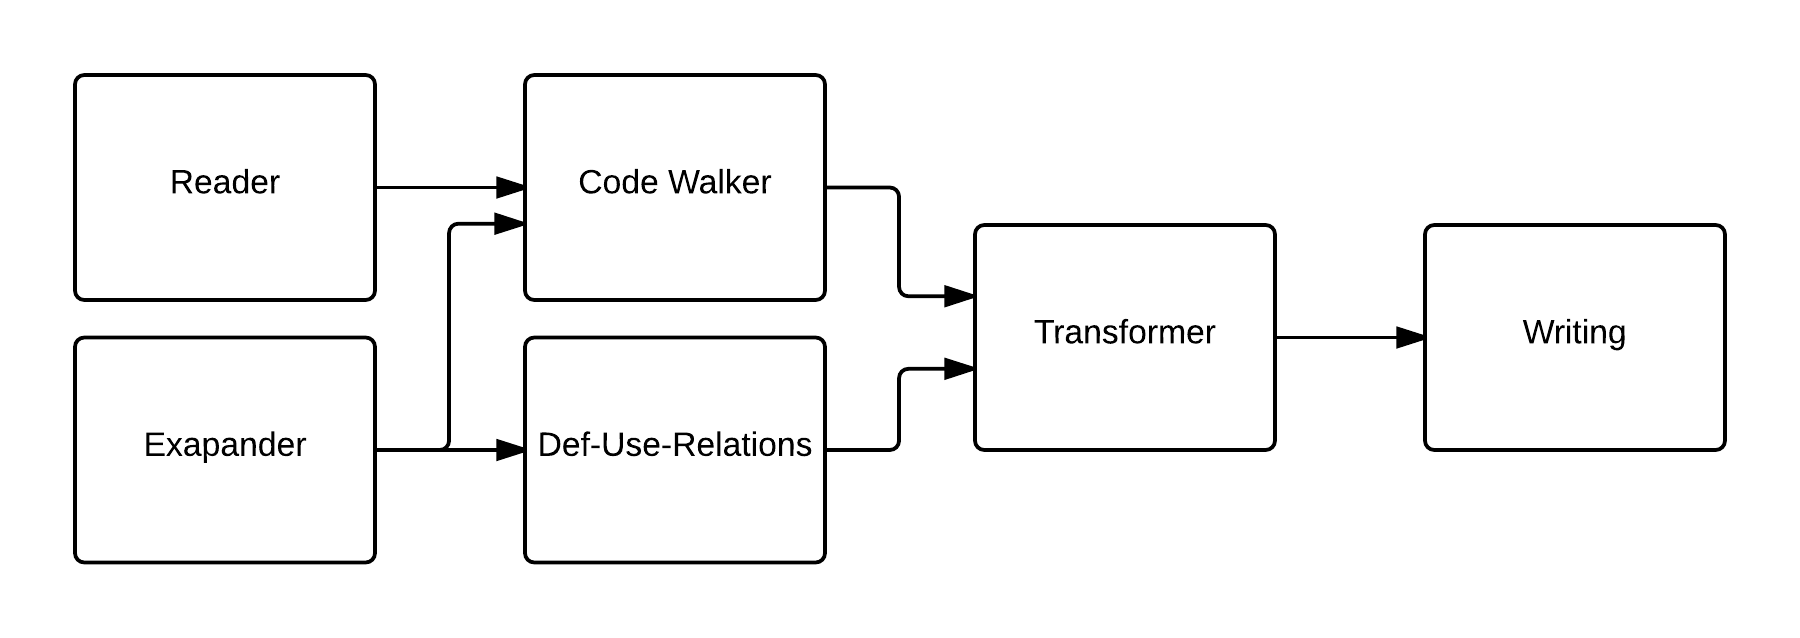
\includegraphics[width=\linewidth]{refactoringTool-arch.png}
\label{architecture}
\caption{Information flow between modules.}
\end{figure}
Figure~\ref{architecture} summarizes the work flow of the refactoring tool where
the Reader produces the non expanded program while the Expander produces the
expanded program. Afterwards the Code walker parses the AST produced by the Reader or the Expander depending the
cases. In order to produce the Def-Use-Relations it is necessary to use the code produced by the
Expander because it has the correct dependency information.
The Transformer uses both information from the Code Walker and the Def Use Relations
to transform the code. Then it goes to the Writing module that produces the output
in the Definitions area.

%The AST is acquired after using the check-syntax button. It was intended to be
%acquired automatically, because DrRacket has an online check syntax, but it was
%not possible. After that it cleans the AST removing information that is not
%necessary, at least for now, for the refactoring operations. When the AST is cleaned it
%passes the exact part of the AST that was selected. And tries to match rules,
%using syntax-parse against that syntax.

\subsection{Syntax Expressions}
%intro and explain the importance of the S-Exp
The s-exp list represent the AST, which provides information about
the structure of the program.
The s-exp list it is already being produced and used by the Racket language and
in DrRacket in order to provide error information to the user.
DrRacket already provides functions which computes the program's s-exp list and uses some of those
functions in the online check syntax and in the check syntax button callback.

%TODO add the functions?


\subsubsection{Syntax Expression tree forms}
DrRacket provides functions to compute the s-exp list in two different formats.
One format is the expanded program, this format is used by the Check Syntax and
the online check syntax, and computes the program with all the macros expanded. %maybe check that
The other format is the non-expanded program and computes the program with the macros
unexpanded.

The expanded program has the macros expanded and the identifier information correctly
computed.
However it is harder to extract the relevant information when compared with the
non expanded program.
%Racket has two forms of syntax tree. An expanded form, with the macros expanded
%and a non expanded form that is after a read-syntax without the macros expanded.

For example, the following program is represented in the expanded program,
and in the non expanded program. %FIXME TODO FIXME change example to a and, or, when or unless

\begin{lstlisting}[basicstyle=\ttfamily, caption="example"]
(and alfa beta)
\end{lstlisting}

\begin{lstlisting}[basicstyle=\ttfamily, caption="Expanded program"]
#<syntax:2:0
 (#%app call-with-values
   (lambda ()
   (if alfa beta (quote #f)))
   print-values)>
\end{lstlisting}

\begin{lstlisting}[basicstyle=\ttfamily, caption="Non-expanded program"]
#<syntax:2:0 (and alfa beta)>
\end{lstlisting}
%Expanded Program Vs Not expanded Program
%Talk about difficulty, durability, Python (other languages)

%[Only in the expanded form] (and) is treated like an if which is bad and give problems
%The rest tends to work.
%testing:
%(if (= (+ 1 2) 1) \#f \#t) to (not (= (+ 1 2) 1))

The expanded program transforms the {\tt and}, {\tt or}, {\tt when}, and {\tt unless} forms into
{\tt if}s which makes refactoring operations harder to implement.

Racket adds internal representation information to the expanded-program which for
most refactoring operations are not needed.

However, the expanded program has important information regarding the binding
information that is not available in the non-expanded form and is rather useful
to detect if two identifiers refer to the same binding.
%TODO check; It also contains information where a program returns or not. TODO CHECK!
In addition, the expanded program has a format that is likely to change
in the future.
Racket is an evolving language and the expanded form is a low level and internal
form of representation of the program.
Additionally we do not consider macros as part of a code that could be refactored,
 since the refactoring tool is targeted at unexperienced programmers macros
will not be used often and therefore it is not considered part of the scope of
this refactoring tool capabilities.

Therefore it is desirable to use the non expanded form for the refactoring %all things considered
operations whenever possible and use the expanded form only for the necessary
operations.
Nevertheless, if we intended to create a tool that gives support to refactoring macros
using the non expanded program would let to errors making the expanded program the
representation of the program used.
Even considering that are no guarantees that would be enough to ensure the correctness of
such refactoring operations due to the reflection capabilities of Racket.


\subsection{Def-Use-Relations}
Def-Use-Relations holds an important information in order to produce correct refactoring operations. %the def-use-relations? holds?
They can be used to check whether or not there will be a duplicated name
or even to compute the arguments of a function to be extracted.
%The information is computed in the online-comp.rkt that is where expands
%and computes the information needed to know the def-use-relations and whether
%the program is syntactically correct.
%There is an online expansion monitor that calls the online-comp, the online-comp
%then expands the program (to the expanded program) and does a trace to get the
%information needed for the arrows (def-use-relations).
%Afterwards it sends back that information to the caller of the online-comp to do
%the replay of the trace did by the compile comp and to process the information
%about the arrows.
%\subsubsection{Def-Use-Relations utility}
DrRacket already uses the def-use-relations in the system and they are visually  %TODO they are or it is?
represented by arrows in the GUI.
The def-use-relations is computed by the online-compiler that runs in the background.
However it is only processed when a program is syntactically correct. (e.g. if
a program has syntax errors there are no arrows produced in DrRacket)

\subsection{Code-walker}
The code-walker is used to parse the syntax tree represented by a syntax elements
that is a list of s-exp in racket. %TODO check this.
A syntax element can contain either a symbol, a syntax-pair, a datum (number, boolean or string),
or an empty list. %might be other stuff but never got it, not relevant?
While a syntax-pair is a pair containing a syntax object as it first element and
either a syntax pair, a syntax element or an empty list as the second argument.
Each syntax-object has information about the line where they are defined and this
information is to search for the correct elements.

%A syntax object combines a simpler Racket value, such as a symbol or pair, with a scope set at each phase level,
%source-location information, syntax properties, and tamper status. In particular, an identifier is represented as
%a syntax object that combines a symbol with scope sets and other information. The lexical information of a syntax
%object is its scope set combined with the portion of the global table of bindings that is relevant to the syntax object’s set of scopes.

Most of the time using the code-walker we are searching for a specific syntax element
and location information contained in the syntax-object  is used to skip the syntax
 blocks that are before the syntax element wanted in the first place.

The Code-walker is a core part of the refactoring tool ensuring that the selected
syntax is correctly fed to the refactoring operations. %actually?

%the way that the code-walker guarantees that goes to every important part of the
%tree is by having a "pointer" to the current selected syntax element, and have
%a stack that contains the remaining code to analyze.
%Because of this structure it is necessary to have a stack in order to search
%the tree correctly and in the best way possible.
%Because Most of the time we are searching for a specific syntax element (e.g function,
%define, etc, because everything is a syntax element in Racket) and using this we
%can skip uninteresting syntax in order to get to the syntax that we want to use.


%%%%%% Writing Part of the Refactoring/refactoring rule
\subsection{Pretty-printer} %output?
%FIXME comments, how to solve this?
Producing correct output is an important part of the refactoring tool.
It is necessary to be careful to produce indented code and we decided to use a pretty-printer
that is already incorporated in the language.
However this pretty-printer does not follow the convention in the {\tt cond} clauses
should be surrounded by [ ] parenthesis. This is not considered a problem because
Racket supports both representations.
One possible solution is to use a different pretty-printer in
order to keep the language convention.

%Some syntax elements (s-expressions) lose some information about parenthesis.
%For example it is a convention that {\tt cond} clauses should be surrounded by [] parenthesis
%but the syntax element does not store that kind of information.
%There are several pretty-printers developed for Racket and even the Racket language
%has one incorporated.
%The one already incorporated does not use the [ ] parenthesis, however racket
%supports both representations.
\subsection{Comments preservation}
Preserving the comment after a refactoring transformation is an important task
of the refactoring tool. If the comment in determined place of the program
changes hits location affecting another structure it could confuse the programmer.
However comment preservation is not implemented yet, making it a limitation of
this prototype.

One possible solution is to modify the syntax reader and add a comment node to the
AST.
While the new node will not be used during refactoring transformations it is used
during the output part of the refactoring operation preserving the comment with
the correct syntax expression.


\subsection{Syntax-Parse}

The Syntax-Parse function provided by Racket is rather useful for the refactoring
operations regarding mainly syntax information.
It provides a wide range of options to help matching the correct syntax with  %fine tunning
backtracking.
The backtracking it is possible to have several rules to be matched
in the same syntax parser, which helps to create more sophisticated rules.

\section{Refactoring operations}
%TODO do introduction
In this section we explain some of the  more relevant refactoring operations and
some limitations of the refactoring tool.

\subsection{Semantic problems}
There are known semantic problems that might occur after doing a refactoring
operation.
One problem occurs when removing the and of the following example.

\begin{lstlisting}[basicstyle=\ttfamily, caption="And example"]
  (and (< 1 (foo 2)) (< (foo 2) 3))
\end{lstlisting}
The refactoring transforms the code into this:
\begin{lstlisting}[basicstyle=\ttfamily, caption="Example"]
  (< 1 (foo 2) 3)
\end{lstlisting}

\begin{lstlisting}[basicstyle=\ttfamily, caption="Foo"]
(define (foo arg)
  (displayln "foo"))
\end{lstlisting}

Instead of applying the side effect that is displaying the the string "foo"
 it will only display the it once. Therefore changing the meaning of the program.

We still kept this refactoring operation because in the vast majority
of the cases this refactoring operation does not change the semantic of the program.
Furthermore, the possible solution would limit excessively this refactoring operation.  %enormously
Considering Racket's reflection capabilities we would only apply this refactoring operation
safely when the arguments of the {\tt and} expression, in this case {\tt < } and the function {\tt foo}
 were datums (number, boolean or string). This line of thought is also applicable to
 the {\tt or} form.


E.g.:
\begin{lstlisting}[basicstyle=\ttfamily, caption="Code sample"]
(if ?x
    (begin ?y ...)
    #f)
\end{lstlisting}
The two different refactoring transformations are possible:
\begin{lstlisting}[basicstyle=\ttfamily, caption="Refactoring option 1"]
(when ?x
      ?y ...)
\end{lstlisting}

\begin{lstlisting}[basicstyle=\ttfamily, caption="Refactoring option 2"]
(and ?x (begin ?y ...))
\end{lstlisting}

The first refactoring option changes the meaning of the program, because if the
test expression, in this case ?x, is false the result of the when expression is \#<void>.
However, the programmer may still want in some situations choose one approach and in others
choose the other one. For example if a programmer is creating a predicate may
choose the {\tt and} version, whereas if the programmer is using another control structure
and do not care for the result of the expression may prefer the {\tt when} version.

\subsection{Extract Function}
Extract function is an important refactoring operation that every refactoring tool
should have.
However there are some concerns to have into account.
In order to extract a function it is necessary to compute the arguments needed
to the correct use of the function.
While giving the name to a function seams quite straightforward it is necessary to
check for name duplication in order to produce a correct refactoring. e.g. having
two identifiers with the same name and in the same scope produces an incorrect program
and therefore modifying the meaning of the program.
Then computing the body and replacing it by the call should be straightforward.
Another problem is where should the function extracted to. A function can not
be defined in an expression, (e.g inside a let) but it could be defined in the top-level
or in any other level that is accessible from the current level.

e.g: When extracting the {\tt (+ 1 2)} to a function where should it be defined?
Top-level? level-0 level-1 or in the current level, level-2?
\begin{lstlisting}[basicstyle=\ttfamily, caption="Extract function levels"]
;;top-level
(define (level-0)
  (define (level-1)
    (define (level-2)
      (+ 1 2))
    (level-2))
  (level-1))
\end{lstlisting}

The fact is that is extremely difficult to know the answer to this question because
it depends on what the user is doing and the user interpretation.
Accordingly we think that the best solution is to let the user decide where
the user wants the function defined.


\subsubsection{Computing the arguments}
%In previous versions of the online-comp information about the type of arrows
%was available in the structure. However, in the recent versions that type of
%information was removed.

%With the previous version of the online-comp the framework was computing the argument for the
%newly extracted function using the type information: "one of 'lexical, 'top-level, 'import".
In order to compute the arguments we have to know in which scope the variables are being defined, in other words,
if the variables are defined inside or outside the extracted function. %FIXME it is weird
The variables defined outside the function to be extracted are the candidates to be the argument %FIXME IMPROVE
of that function.
However, imported variables, whether from the language or from other libraries
does not have to be passed as arguments, to solve this we considered two possible solutions:

  -Def-use-relations + Text information

  -Def-use-relations + AST

The first approach is simpler to implement and more direct than the second one.
However, it is less tolerant to future changes and to errors.
The second one combines the Arrow information with the syntax information to
check whether it is imported from the language or from other library.

We choose the second approach in order to provide a more stable solution to compute
 correctly the arguments of the new function.

\subsection{Let to Define} %implemented is it worth it?
%Refactoring Let to Defines Usefulness Vs implementation difficulty

%there are several let forms, we want to focus on let* let and named let.
We noticed the similarity of a {\tt let} expression with a function, therefore making
it easy to choose one of them by mistake.
Therefore we decided to provide a refactoring operation that would make that transition simpler.

There are several let forms, but we want to focus in the ones more similar to
a function, namely {\tt let}, {\tt let*}, and {\tt named let}.
The ones that closely represent a function is the  {\tt let} and the {\tt named let}
because of the difference between the {\tt let} and {\tt let*} evaluate their
values expressions.
The {\tt let} defines variables independently, while {\tt let*} can use the value of the variable defined before.

The {\tt let} and the {\tt named let} can be directly mapped to a function, however the {\tt named let}
 can be directly mapped to a define whereas the {\tt let} can only be directly mapped
to an anonymous function.
However, we did not consider the transformation of a {\tt let} to an anonymous function, {\tt lambda},
making the code simpler and therefore it was not implemented yet.\\


However, the refactoring operation that transform a {\tt named let} into a {\tt define} function,
 could have syntax problems because a {\tt let} form can be used in expressions, but the {\tt define} can not.
In the vast majority of cases this refactoring is correct, but when a let is used in an expression
it is not correct and it changes the meaning of the program, transforming a correct
program in a incorrect one.
e.g.
\begin{lstlisting}[basicstyle=\ttfamily, caption="Let in an expression"]
(and (let xpto ((a 1)) (< a 2)) (< b c))
\end{lstlisting}
Modifying this {\tt named let} into a define would raise a syntax error because a
define could not be used in an expression context.
This could be solved by using the local keyword that is an expression like
the let form.
However, the local is not used very often and can confuse the users.
This reason made us keep the refactoring operation without the local keyword that works for
most of the cases.



%\subsection{Define to Let} %not yet implemented
%Refactoring Define to Let Usefulness Vs Implementation difficulty
%TODO implement.
%Useful for when changing several defines and merging them into a let.
%the let would "swallow" all the range of the defines scope
%Interesting?

%It would be let* and named let* If define is a function it does not work.
%Is that worth it?

\subsection{Wide-Scope Replacement} %is this a feature or a refactoring?
The Wide-Scope replacement brings the possibility to replace all the duplicated
code with a function call. This is usually performed after an extract function refactoring.
%The Wide-Scope Replacement brings an huge improvement on the utility of the refactoring regarding the use
%of the extract function refactoring operation.

The Wide-Scope replacement refactoring operation searches for the code that is duplicated of the extracted function and then it replaces for the call of the
extracted function and it is divided in two steps: %FIXME Improve

- Detect duplicated code

- Replace the duplicated code

Replacing the duplicated code is the easy part, however the tool might has to compute %have?
the arguments for the duplicated code itself. The argument computation occurs when
the code is the same, but it has different variable names. This is not yet in this
version of the refactoring tool. %TODO rewrite, it is buggy

\subsubsection{Detecting duplicated code}
Correctly detect code duplication is a key part for the correctness of this refactoring.
Even the simplest form of duplicated code detection, when it only detects code duplication
when the code is exactly equal, may have some problems regarding the bindings.
For example, if the duplicated code is inside a let that changes some binding that must
be taken into consideration.
Racket already provides functions that compute if the bindings are the same.
However that does not work if we consider the program in the not expanded
form because there is not enough information for those bindings to work. %FIXME improve :(

%[TODO Recently racket changed binding expansion and it brought interesting improvements to racket and that might be useful for this, read paper before]

Therefore, in order to compute the correct bindings, it is necessary to use the expanded form
of the program.

The naive solution is to use the expanded program to detect the duplicated
 code and then use this information to do the replacing of the duplicated code.
However when expanding the program Racket adds necessary internal information to
run the program itself that are not visible for the user.
While this does not change the detecting of the duplicated code, this adds unnecessary information
that would have to be removed. %FIXME
In order to solve this problem in a simple way we can use the expanded code to detect
the correctly duplicated code and use the non expand program
to compute which code will be replaced.

However this detection is a quadratic algorithm which might
have some performance problems for bigger programs. %TODO TODO TODO

Detecting duplicated code can be added to the automatic detection of possible refactoring operations to be applied. %FIXME is this already done?
Notifying the users of a possible extract function operation if there is duplicated code.
This is a rather useful notification because for programs that are bigger than the
visible part of the screen.
Which might be difficulty for the user to remember if a piece of code was duplicated or not.


%This runs after detecting the duplicated code, so the bindings are corrected identified.



%\subsection{Implemented Refactoring Operations:}
%Is this worth it?

\section{Features}
This section describes some of the features that improve the utility of this
refactoring tool to beginner programmers. %TODO shall I name them?
\subsection{User FeedBack}
It is important to give proper feedback to the user while the user is attempting or
preforming refactoring operations.
By previewing the outcome of a refactoring operation is an efficient form to
help the users understand the result of a refactoring before even applying the refactoring. %FIXME or understand what a refactoring operation is/do
Previewing works by applying the refactoring operation in a copy version of the AST
and displaying those changes to the user.
It was also studied the possibility of giving feedback to the user instead of
just disabling the refactoring operation button when the tool could not perform the refactoring operation.
The tool should provide information about the steps needed in order to be possible to apply
 that refactoring operation.
However, after an analysis it was clear that these situations rarely occur
in Racket language and therefore it was not implemented.


\subsection{Automatic Suggestions}
Beginner programmers usually do not know which refactoring operations exist or
which can be applied.
By having a automatic suggestion of the possible refactoring operations available
 the beginner programmer can have an idea what refactoring operations can be
 applied or not.

In order to detect possible refactoring operations it parses the code from the
beginning to the end and tries to check if a refactoring is applicable.
To do that it tries to match every syntax expression using syntax parse.
In other words it uses brute force to check whether a expression can be applied
a refactoring operation or not.

To properly display this information it highlights the source-code indicating
that there is a possible refactoring.
This feature could be improved by having a set of colors for the different types
of refactoring operations.
Moreover, the color intensity could be proportional to the level
of suggestion. (e.g the recommended level to use extract function refactoring
increases with the number of duplicated code found) %maybe produce an example?


\section{Analysis}
%It was made an analysis to compare the refactoring tool with the others
%table information is available in GIT repository
%what my tool is different, what it is equal
\begin{table}[]
\centering
\caption{Data Structures}
\label{my-label}
\begin{tabular}{c|c|c|c|c}
Name       & AST & PDG & Database & Others \\ \hline
Griswold   & X   & X   &          &        \\ \hline
HaRe       & X   &     &          &        \\ \hline
Rope       & X   &     & X        &        \\ \hline
Bicycle    & X   &     & X        &        \\ \hline
Pycharm Edu & X   &     & X        &        \\ \hline
Javascript &     &     &          & X
\end{tabular}
\end{table}

The table summarizes the data structures of the refactoring tools deeply analyzed.
It is clear that the AST of a program is an essential part of the refactoring
tool information with every refactoring tool having an AST to represent the program.
Regarding the PDG and Database it has mainly information about the def-use-relation
of the program. The PDG has also control flow information among others.

HaRe only uses the AST as a source of information of the program. Thus, by not having
the def-use-relation or a PDG it has less information to perform the refactoring operations.
However, because HaRe is for the Haskell program language that is purely-functional
programming language that extra information is not necessary to perform a good set of
refactoring operations correctly.



Our implementation uses the same data structures, the AST and
def-use-relations. The def-use-relation is often represented as a database,
some refactoring tools annotate that information in the AST, %haskell v2
some tools extract the information from the AST itself when it is possible and
it is possible to extract that information from the PDG.


Some tools have more information about the program, either because they need that
information to perform the refactoring operation or because they need to prove that
the refactoring is correct.  %case of pycharm/python && Griswold

%Undoubtedly the main difference is in the objectives of each refactoring tool.
Some tools like the one build by Griswold focus on the correctness of the refactoring
operations.
Others, focus in offering refactoring operations for professional or advanced users.
However, the goal of our refactoring tool is to provide refactoring operations
designed for beginners. %FIXME suited aimed targeted
Therefore we are not interested in refactoring operations formerly proven %FIXME REWRITE
correct or provide refactoring operations only used in advanced and complex use cases. %FIXME where is the comma??
We intend to have simple, useful, and correct refactoring operations for the usual use cases a beginner would use.
With this set of scope we exclude macros usage, classes and other complex structures %TODO check this!
not used by beginners.

%TODO add I already used the refactoring tool to do a refactoring operation in
%the source code of the refactoring tool. However this is only applicable in the parts that are supported by this refactoring tool.

\section{Evaluation}
Case Study: (find a good ones) FP Project, Architecture Project. For SLATE
Correctness: Here?
\section{Conclusion}
def-use-relations + AST is sufficient.

Importance of some refactoring operations

Maintainability of the refactoring tool?

Framework?
\section{Future work}
Detect when a developer is refactoring in order to help the developer finish the
refactoring by doing it automatically.
Improving automatic detection
Wide-scope-replacement smarter and better, computation of the arguments
Improve the Preview of the refactoring operations.

%\section{FrameWork}
Python: [framework]
One of the goals of this thesis is to create refactoring for dynamic languages in general,
in other words, to create a Framework for refactoring tools.
//by using the same structure (program, framework, choose one better)
After creating several refactoring operations for Racket Python was chosen next.
POC (prove of concept)
It was created a prove of concept in Python consistent in several refactoring operations, such as:
[TODO] say which refactoring operations were implemented.
Python was chosen because there is already an implementation of Python for the
 DrRacket environment in which the refactoring tool for Racket was first developed.

%[TODO say what parts of the code were reused]

 %[TODO Explain META-LANGUAGE]
 The implementation for DrRacket is what does the trick, because by implementing
 the language with Racket syntax we are basically using as a meta-language that
 can represent several languages. Being the meta-language a language that are
 composed only by syntax elements is a huge advantage to compute effortless new
 refactoring operations for new languages when compared with the necessary effort to create
 the refactoring operations directly for that language.

\subsection{Statement based languages}
This Framework was build with a base of expression based languages. The flow of
the program is needed to decide whether or not a refactoring can be correctly done
or even to decide where and how many returns a function needs. However this could
be minimized with a PDG (program depedence graph) that has the control flow information
needed to compute correct refactorings.

\section{Features}
how easy it is to add new refactoring operations and languages
The framework it is simply to use, it is only necessary to have a specification file
of each refactoring operation.
That file must have a function that receives two arguments,
one is the AST of the program and the other is the def-use-relation.
This information makes it possible to have several refactoring operations that help
the programmer.
what was "reused"
everything except the refactoring operations itself.
the advantages of that
This Framework makes it easier to implement refactoring operations for dynamic languages,
with only the catch that they have to be implemented for DrRacket. Helping minimizing
the problem of the difficulty and lacking of refactoring operations for dynamic languages.
(for at least every language implemented for DrRacket)

\section{Analysis}
\subsection{Famix}


\section{Future Work}
Add a PDG to the framework.


%%!TEX root = ../report.tex

% 
% Architecture
% 

%(DrRacket helps with this by giving an access to the bindings for a correct program, I do not have to compute that, which is awesome!)
%it is not an intention to care about refactorings regardint meta-programming or reflection calls. Even the Static object oriented refactoring tools with all their refactoring operations, developers do not try to solve that problem.

\section{Future Work}
%DrRacket Image
%\begin{figure}[tbhp]
%	\centering
%	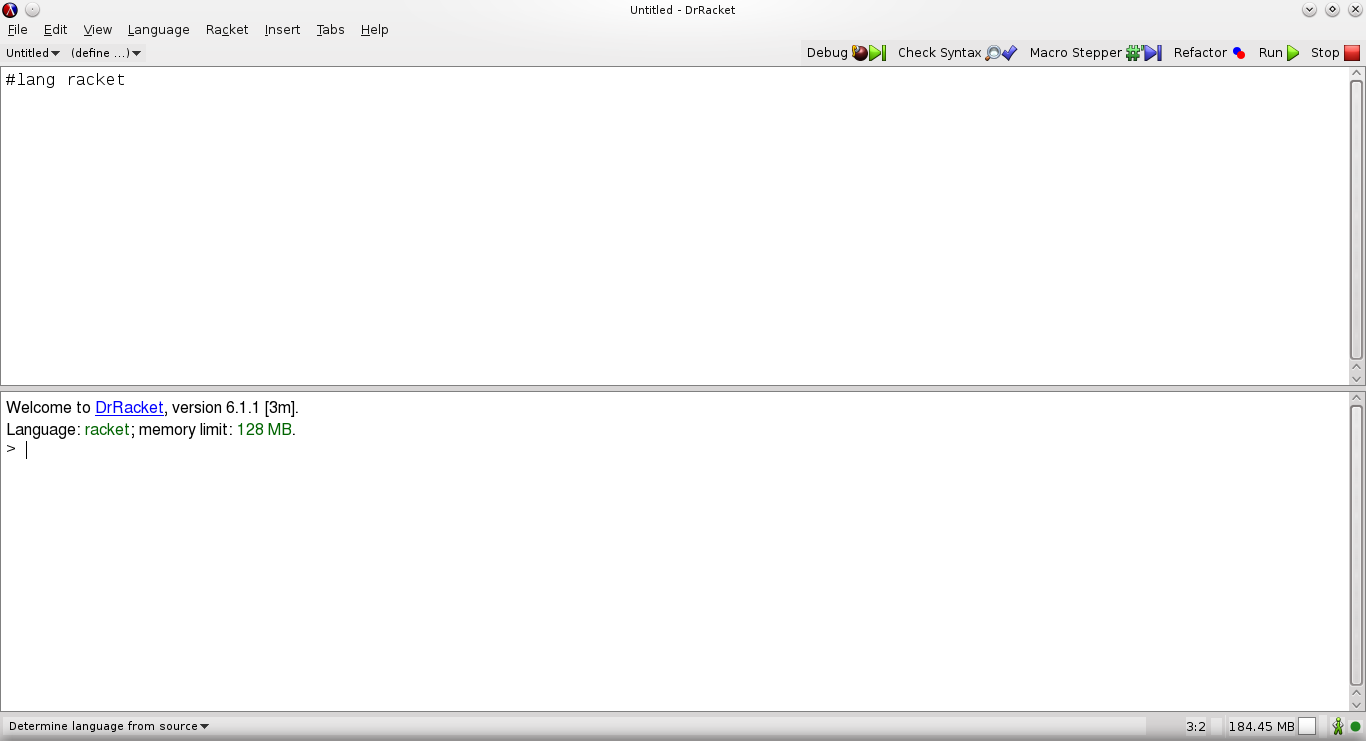
\includegraphics[width=1\textwidth]{img/DrRacketGui.png}
%	\caption{DrRacket Graphical user interface}
%	\label{fig:DrRacketGui}
%\end{figure}


%Base de dados preenchida durante a compilacao, que se presenta em forma de setas que eu vou usar para resolver os problemas semanticos.
%Seccao de critica/analise. 



%whereas Python is a very high-level programming language that supports the imperative, functional and object-oriented programming paradigms and is very popular in many areas.
The objective is to create a refactoring tool, for Racket in the DrRacket IDE, that helps and motivates unexperienced users to use refactoring operations. Racket is known for being used as an introductory programming course and DrRacket IDE is known as a pedagogic environment.

Besides being a simple and a good IDE to learn how to program, DrRacket gives some functionalities that are helpful to the programmer of the refactoring tool. 
DrRacket has a database filled during compile time that has information about all the bindings of each variable and DrRacket represents it in the visual form of arrows. 
Each arrow knows where is pointing to and where is the beginning of itself. 
This is rather helpful for the refactoring operations that need semantics.
For example, for the extract-function it makes it very easy to know what variables will be arguments of the extracted function and what variables are not needed to be passed as arguments.

DrRacket also has syntax objects. These objects have all the information regarding the syntactic information and their location. Basically they represent an annotated AST with the location of each object.

%By having this features it is possible to create a tool that helps the unexperienced users and it is useful for more experienced users.



%\input{sections/7-evaluation.tex}
%%!TEX root = ../report.tex

% 
% Conclusions
% 

\section{Conclusions}

%refactoring is used a lot
%BUT tools are underused.
% lack of dynamic refactoring tools and operations when compared with static object oriented ones. some of that exist are dead.
% Intention of creating a tool for unexperienced users to start doing refactoring operations with the tool.


Refactoring operations are important in order to maintain the quality of the software but because they are error prone and time consuming, refactoring tools are needed.
The objective of this overview is to show what exists regarding refactoring tools for dynamic languages and the difference between those tools and tools made for static object oriented languages.

%Although almost every tool made for static object oriented languages has the refactoring operations for 90\% of the refactoring operations used by the users, but in the best case scenario only 27\% of the refactoring operations were tool assisted.

Although almost every tool made for static languages supports 90\% of the refactoring operations, the users only use refactoring tools for 27\% of the cases. %showing that the major part of the refactoring operations are done manually]

This survey also shows how few refactoring operations exist in general for dynamic languages and why it is more difficult to make a refactoring tool for dynamic languages.

In conclusion, this paper shows the importance of having a refactoring tool concerned about the unexperienced users. 
Besides having dynamic languages as the recommended languages to learn how to program, the dynamic languages are growing. 
And that tool might help the users start to use the refactoring tools and refactoring their programs alongside with programming.

%and to show the need of a refactoring tool for dynamic languages targeted for unexperienced programmers

%\end{multicols}
%\newpage




%
% Bibliography
%
\bibliographystyle{unsrt}
\bibliography{example.bib}
%\newpage
%\appendix
%%!TEX root = ../report.tex

\section{Appendix} % (fold)
\label{sec:attachments}


% replace example.bib with your .bib


\end{document}
